\documentclass[12pt, a4paper,oneside,twocolumn]{article}
%Peter Armstrong
\title{Search}
\author{Peter Armstrong}


\usepackage{graphicx}
\begin{document}
\maketitle

\abstract{Abstract goes here}
The object of this research was to develop a simple information retrieval program or \emph{search engine}. A program was developed that indexed the files to be searched based on the words contained in the files. This enabled efficient searching for multiple search terms over a large number of documents. The recall of this search engine needs to be improved before the program is useful in anything but the most trivial search scenario.




\section{Introduction}
Searching files for a words is a fundamental computing operation. There is a file searching tool built in to every operating system and efficient search is vital to the internet. 
A simple information retrieval system will be designed to search a collection of documents for a number of keywords. The system will identify each document that contains some or all keywords, and prints the location of the files in descending order, sorted by the number of keywords found. The number of occurrences of a particular word will be a ranking factor.

\paragraph
\noindent
Knuth \cite{knuth} states that `\emph{searching is the most time consuming part of many programs, and the substitution of a good search method for a bad one often leads to a substantial increase in speed}'.
There  has been extensive work done in the field of search and many companies consider their search algorithms a trade secret. There are also open-source search systems such as the Apache Lucene library \cite{lucene} which are freely available to use, study and modify.

\section{Theory}

There are many ways to approach this problem but two will be discussed in detail:

\subsection{Forwards Indexing}
A map structure is used with the document names being stored as the keys and the words in the document stored as values associated with the keys. The advantage of this method is that it is simple and quick to add new files to the index.  Adding a file to the index has constant complexity.
To search for a word using this system, each key-value pair must be accessed to see if the document contains the word being searched for. The complexity is directly proportional to the size of the document being searched. It is also directly proportional to the number of search terms. This results in a complexity of O(n) when searching for one word, and O(n\textsuperscript{2}) when searching for  more than one word.

Because adding a file to the index is quick, this method is suitable for searches when the data to be searched changes regularly. The disadvantage of this method is the time complexity is high when searching a large number of files, and increases quickly if a number of terms are to be searched for.

\subsection{Inverted Index}
An alternative way to search is by using an inverted index \cite{invertedindex}. This involves creating an index of all the words that are contained in each file to be searched. 

Each word is saved as the key in a map structure. The list of files where the word appears are saved as the value associated with this key.
The complexity of the initial indexing of the files to be searched is linearly proportional to both the number of files and the number of words contained in the files.
Searching for a word using this system is fast as the words can be directly accessed and their respective values can be shown. 

%The result set must then be sorted 
%The result set can then be sorted based on the number of values. complexity of the sorting of the results is O(nlogn). As the number of results is likely to be much less than the number of files in the total data set, the sorting operation is typically very fast.

\subparagraph  
\noindent
Although it takes some time to initially index the files to be searched, once the index has been created searching is very quick. This method is preferred when the data set to be searched is large and does not change regularly, or when there are a large number of searches to be run on the same data set.

\section{Method}
\subsection{Indexing}
The method chosen for this paper was an inverted index. When the files to be searched are chosen, the files are each opened. Each new word found in the file is added to a map structure as the key. The location of each file that contains that word is then added to the bucket relating to that key. The bucket is implemented using a list structure. 

\subsection{Searching}
The list of search terms is iterated through. For each term,  the corresponding map entry is accessed using the search term as the key. If the key is found, the corresponding list of values is returned and added to a list structure. 

The files are then added to a map structure as key and the frequency of the search terms in the file is added as the corresponding value.
The map structure is then sorted based on it’s values. The sorting operation has complexity O(nlogn). As the result map is typically much smaller than the full data set, this is typically a very quick operation.

\section{Results}

Both indexing and searching performance was tested for a variety of different cases.

\subsection{Indexing time vs File Size}

Single files of different words were indexed and the time taken to index them was recorded. The graph (Figure 1) shows that the time taken to index increases linearly with file size.

\begin{figure}[htp]
\centering
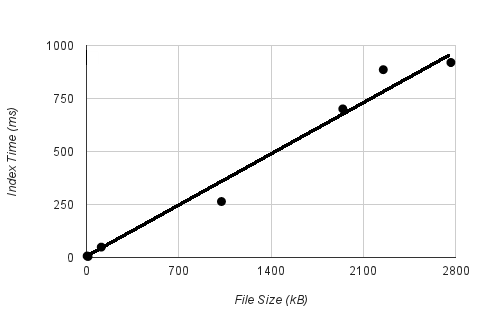
\includegraphics[scale=0.45]{sizevstime.png}
\caption{File Size vs Index Time}
\label{}
\end{figure}


\subsection{Indexing time vs Number of Files}

A dictionary of words was split into equal text files, each containing 500 words. For various numbers of files, the time taken to index them was plotted against the number of files being indexed. The graph shows that the time to index also increases linearly with the number of files.
\begin{figure}[htp]
\centering
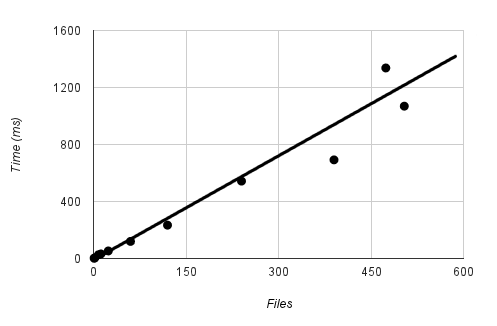
\includegraphics[scale=0.45]{filesvstime.png}
\caption{Number of Files vs Index Time}
\label{}
\end{figure}

\subsection{Search Terms vs Search Time}
The dictionary of words split into a number of equal files was again indexed. A different number of terms was searched for and the time taken to run the search was plotted against the number of search terms. To ensure different files were being accessed, a word starting with each letter in the alphabet was used.
The original complete dictionary was also tested in this way, and the results are show on the bottom (red) graph of Figure 3.
\begin{figure}[htp]
\centering
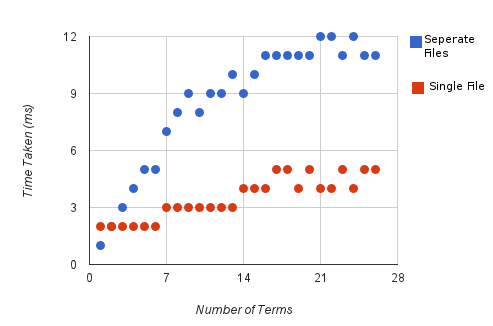
\includegraphics[scale=0.45]{searchTermsvstime.png}
\caption{Search Terms vs Search Time}
\label{}
\end{figure}

Based on this small set of data, the graphs appear to have logistic progression. It takes a considerably longer time to access search results if they are spread across a number of smaller files rather than in one large file.

\subsection{Recall}
According to Langville and Meyer \cite{google}, search engine recall is the ratio of the number of relevant documents to the total number of documents in a collection. 

The search engine was tested on the Medlars test collection \cite{medlars} for the phrase `neoplasm immunology'. There are 24 documents relevant to this search phrase in the Medlars collection. This search engine returned only three documents, giving it a recall ratio of 3/24=0.125. This is partly because the search engine does not do any pre-processing of the search terms. The search engine only returns matches of the exact search term; plurals, uppercase letters, different tenses or words that contain punctuation will not be found. The recall ratio was increased to 12/24 = 0.5 when the terms `neoplasms', `neoplasm,', `immunology' and `immunology,' were added to the search.

\section{Conclusions}
A simple search engine with an efficient search manner was designed. The bottleneck in this system is the amount of time needed to index a large dataset. While the search is relatively quick, the accuracy or recall of the search engine needs to be improved before it can be used in any but the most trivial situations.


\section{Further Work}

The search recall of the system could be greatly improved by doing some pre-processing to the search terms. Approximate string or `fuzzy' matching of the search terms could be included to provide a more useful system.

The retrieval of phrases could be improved. Currently the system does not take account of the position of the search terms in the file. A file containing words written as a phrase will rank the same as a file that contains words that are not beside each other. This could be improved by indexing the position of each word in the document.

\begin{thebibliography}{9}
\bibitem{knuth}
Knuth, D. E. 1998 \emph{The Art of Computer Programming- Searching and Sorting} 2nd ed. Reading, Massachusetts. Addison Wesley Longman.

\bibitem{lucene}
apacehelucene
"http://lucene.apache.org/core/"

\bibitem{invertedindex}
"http://nlp.stanford.edu/IR-book/html/htmledition/a-first-take-at-building-an-inverted-index-1.html"

\bibitem{javaCollection}
java collection api
"http://docs.oracle.com/javase/1.4.2/docs/api/java/util/Collections.html"

\bibitem{google}
Langville, A.N., Meyer, C.D. 2006 \emph{Google's PageRank and Beyone} Princeton, New Jersey. Princeton University Press.

\bibitem{medlars}
"http://web.eecs.utk.edu/research/lsi/corpa.html"

\end{thebibliography}

\end{document}
